\documentclass{standalone}
\usepackage{graphicx}	
\usepackage{amssymb, amsmath}
\usepackage{color}

\usepackage{tikz}
\usetikzlibrary{intersections, backgrounds, patterns, patterns.meta}
\usepackage{pgfmath}

\definecolor{light}{RGB}{220, 188, 188}
\definecolor{mid}{RGB}{185, 124, 124}
\definecolor{dark}{RGB}{143, 39, 39}
\definecolor{highlight}{RGB}{180, 31, 180}
\definecolor{gray10}{gray}{0.1}
\definecolor{gray20}{gray}{0.2}
\definecolor{gray30}{gray}{0.3}
\definecolor{gray40}{gray}{0.4}
\definecolor{gray60}{gray}{0.6}
\definecolor{gray70}{gray}{0.7}
\definecolor{gray80}{gray}{0.8}
\definecolor{gray90}{gray}{0.9}
\definecolor{gray95}{gray}{0.95}

\begin{document}

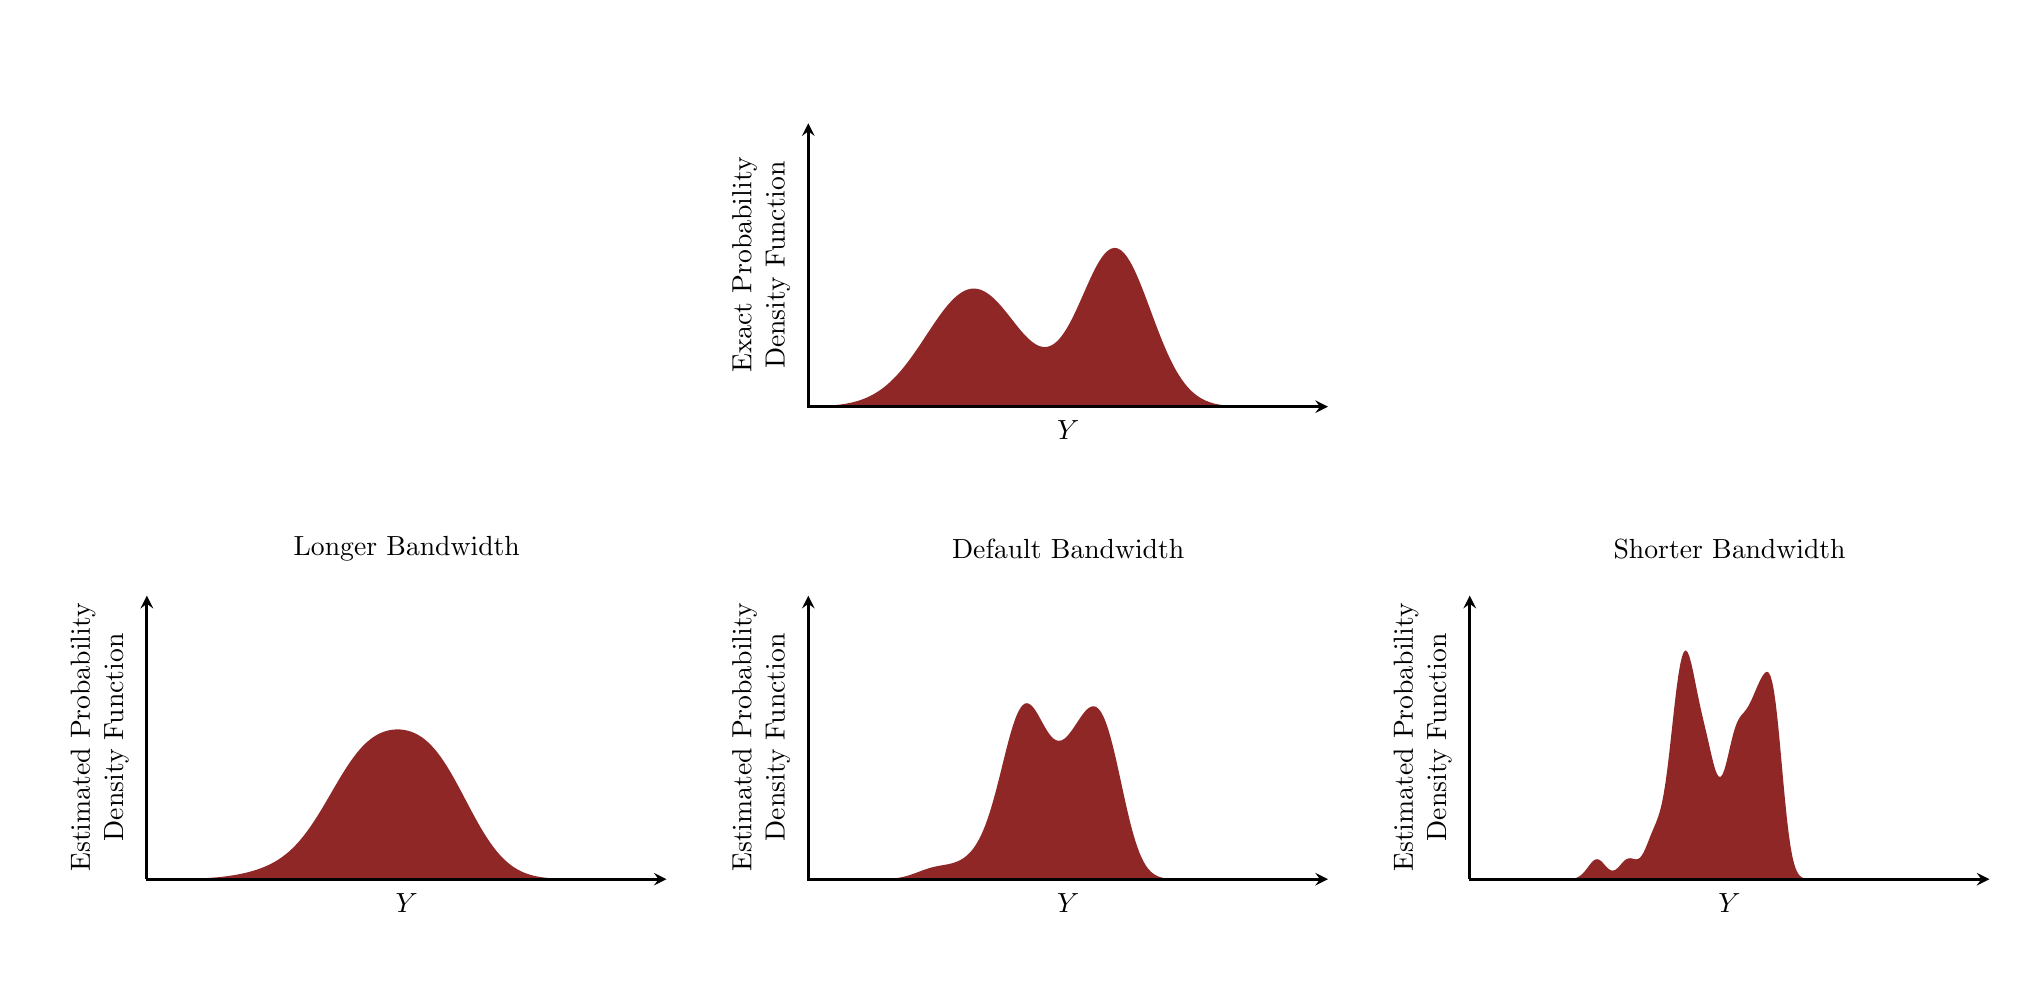
\begin{tikzpicture}[scale=0.3, thick]

\pgfmathsetmacro{\hscale}{2};
\pgfmathsetmacro{\vscale}{30};

\begin{scope}[shift={(0, 0)}]
  \draw[white] (-16, -4) rectangle (12, 16);

  \fill[domain={-5:5}, smooth, samples=150, line width=1, variable=\x, color=dark] 
    plot ({\hscale * \x},{5 * (exp(-0.5 * (\x - 1) * (\x - 1) / (0.75 * 0.75) ) / 0.75 + exp(-0.5 * (\x + 2) * (\x + 2) / (1 * 1) ) / 1)});
  
  \draw [->, >=stealth, line width=1] (-11, 0) -- (-11, 12);
  \node[rotate=90, align=center] at (-13, 6) { Exact Probability\\Density Function };
  
  \draw [->, >=stealth, line width=1] (-11.05, 0) -- (11, 0);
  \node at (0, -1) { $Y$ };
\end{scope}

\begin{scope}[shift={(-28, -20)}]
  \draw[white] (-16, -4) rectangle (12, 16);

  \fill[dark, line width=1] (-11, 0) 
    \foreach \y [count=\n] in {6.25756192297106e-05, 7.61723599346208e-05, 9.83126696176251e-05, 0.000126093925080871, 
                               0.000160425573826446, 0.000202707318371844, 0.000254597275519045, 0.000317308073458524, 
                               0.000392740126946637, 0.000483306913298671, 0.000590407149442086, 0.000716350486209304, 
                               0.00086438194883991, 0.00103584358946351, 0.00123324145172332, 0.0014606635063618, 
                               0.00171909879471016, 0.00201105699870865, 0.00234137573826529, 0.00271065551266824,
                                0.0031214865317438, 0.00357916577359727, 0.00408466354952629, 0.00464084271783677, 
                                0.00525403508882421, 0.00592647733951645, 0.00666209176601354, 0.0074694058825731, 
                                0.00835326715775148, 0.00931969407759692, 0.0103808153127038, 0.0115455343153368, 
                                0.0128226023015616, 0.0142285818241539, 0.0157772924251011, 0.0174795224142089, 
                                0.0193554496136104, 0.0214231997337807, 0.0236927844847509, 0.0261847020074193, 
                                0.028918555790701, 0.0318986117850302, 0.0351399933177906, 0.0386585869829904, 
                                0.0424469850459357, 0.0465082599660789, 0.0508478814935813, 0.055442300938852, 
                                0.0602774976878318, 0.0653422685262621, 0.0705967841933453, 0.0760093973141608, 
                                0.0815489682574561, 0.0871654562030382, 0.0928151224601537, 0.0984489558396286, 
                                0.104018160370314, 0.109476300969828, 0.114768413502665, 0.119856067301672, 
                                0.124702943881071, 0.129262215167272, 0.133512724917167, 0.137438108521772, 
                                0.141010042358985, 0.144226285490663, 0.147092700872022, 0.149601551733711, 
                                0.151764560325025, 0.153603270948066, 0.155123634135455, 0.156341187868633, 
                                0.157280961608173, 0.157950554840728, 0.158357809645787, 0.158519674392788, 
                                0.158434759335033, 0.158095088941126, 0.157504770623227, 0.156649989871368, 
                                0.155505840650171, 0.154068347189544, 0.152317000145352, 0.150216715354279, 
                                0.147767368897714, 0.144953743624231, 0.141742862000883, 0.138151294116272, 
                                0.134179729976398, 0.12981484833615, 0.125092404854429, 0.120036361564059, 
                                0.114662240128508, 0.10902178978801, 0.103160452894451, 0.0971198373883553, 
                                0.0909599867091084, 0.0847369358063988, 0.0785068623894771, 0.0723274765461836,
                                0.0662505598471219, 0.0603316388166764, 0.0546165892035836, 0.0491400422226428, 
                                0.0439438936827146, 0.0390568032586257, 0.0344897241993762, 0.0302642410515209, 
                                0.026391469115136, 0.0228597339770105, 0.0196707234620412, 0.0168216888717627, 
                                0.0142850543988192, 0.0120480955495882, 0.0100997618705871, 0.00840547855129225, 
                                0.00694542076083244, 0.00570557950906227, 0.00465220258180702, 0.00376471153495138, 
                                0.00302994831474104, 0.00241989806992675, 0.0019173974111845, 0.00151142151939013, 
                                0.00118213595325468, 0.000917045510522518, 0.000707738438138116, 0.000542012200640313, 
                                0.000411598089969919} {
    -- ({-10.24479 + 0.1311402 * (\n - 1)} , 40 * \y)                         
  };
   
  \draw [->, >=stealth, line width=1] (-11, 0) -- (-11, 12);
  \node[rotate=90, align=center] at (-13, 6) { Estimated Probability\\Density Function };
  
  \node at (0, 14) { Longer Bandwidth };
  \draw [->, >=stealth, line width=1] (-11.05, 0) -- (11, 0);
  \node at (0, -1) { $Y$ };
\end{scope}

\begin{scope}[shift={(0, -20)}]
  \draw[white] (-16, -4) rectangle (12, 16);

  \fill[dark, line width=1] (-9, 0) 
    \foreach \y [count=\n] in {0.000118857037915087, 0.000157250837610117, 0.000225104162409555, 0.000317183246841441,
                               0.000440526676099045, 0.000601407512773053, 0.000807981501596002, 0.00106987628555737, 
                               0.00139322994538596, 0.00178553931409196, 0.00225509772301435, 0.00280260855921128, 
                               0.00342896471386685, 0.00413437946306718, 0.0049087352305581, 0.0057416476397614, 
                               0.00662032616292913, 0.00752486117871137, 0.00843604650770841, 0.00933255359372601, 
                               0.0101946779078866, 0.0110058673594553, 0.0117505235766375, 0.0124222554811916, 
                               0.0130202204543976, 0.013547135714044, 0.0140159303293998, 0.0144441669567538, 
                               0.0148528662985067, 0.0152681596194561, 0.0157165708073101, 0.0162271395188833, 
                               0.0168289898885938, 0.0175474657512708, 0.0184123052132412, 0.0194536397772649, 
                               0.0206954565332241, 0.0221712979332786, 0.0239203284291439, 0.0259715314621071, 
                               0.028368547274916, 0.0311669787873975, 0.0344007081498683, 0.0381199762670147, 
                               0.0423913708761425, 0.0472381713214122, 0.0526973029327275, 0.0588220429395926, 
                               0.0655954589753159, 0.073009748985145, 0.0810601218290846, 0.089662824711452, 
                               0.0987335974962169, 0.108170708476513, 0.117816126920463, 0.127505312875338, 
                               0.137045210524108, 0.146233628211453, 0.154875637371485, 0.162751465484242, 
                               0.169686690593369, 0.175544826095374, 0.180176655632667, 0.183512914912406, 
                               0.185550564593786, 0.186281235529602, 0.185775346647959, 0.184173719284676, 
                               0.181608416926502, 0.178261453495942, 0.174357181126901, 0.17010243978079, 
                               0.165720012709535, 0.161424011623487, 0.157406369997016, 0.153853939375172, 
                               0.150891338191294, 0.148625940294688, 0.147156726549326, 0.146486786112117, 
                               0.146616042789375, 0.147543993812519, 0.149174151307741, 0.151425042478282, 
                               0.15421538901415, 0.157407103941331, 0.160879180164438, 0.164507690887224, 
                               0.168153177434165, 0.171686471773201, 0.174965624231423, 0.177859018895083, 
                               0.180241239096294, 0.181961936448976, 0.182898327222944, 0.182944157338261, 
                               0.181965208307522, 0.179872068450774, 0.176619389698331, 0.172143060778176, 
                               0.166436850304743, 0.159566183586944, 0.151588410715655, 0.142615674418503, 
                               0.132830924786773, 0.122408687827048, 0.111556731658474, 0.100510344694643, 
                               0.0894866271071343, 0.0787105295426204, 0.0683665614023804, 0.0586167954858202, 
                               0.0496204404353945, 0.0414406901754424, 0.0341303493532968, 0.0277478172693981, 
                               0.022238197817191, 0.0175618249377324, 0.0136889861614447, 0.0105129074325043, 
                               0.00795000997872809, 0.00593369011472522, 0.00436221578492737, 0.0031557069453416, 
                               0.00225308413977176, 0.00158442318027234, 0.00109570298946802, 0.000747737393476522, 
                               0.000502728703429897} {
    -- ({-7.978874 + 0.09566594 * (\n - 1)} , 40 * \y)                         
  };
   
  \draw [->, >=stealth, line width=1] (-11, 0) -- (-11, 12);
  \node[rotate=90, align=center] at (-13, 6) { Estimated Probability\\Density Function };
  
  \node at (0, 14) { Default Bandwidth };
  \draw [->, >=stealth, line width=1] (-11.05, 0) -- (11, 0);
  \node at (0, -1) { $Y$ };
\end{scope}

\begin{scope}[shift={(28, -20)}]
  \draw[white] (-16, -4) rectangle (12, 16);

  \fill[dark, line width=1] (-9, 0) 
    \foreach \y [count=\n] in {0.000238214037688607, 0.000373356853394448, 0.000655923816373923, 0.00110456687328344, 
                               0.00178300718133454, 0.00276132764927196, 0.00409787188692109, 0.00582724379848738, 
                               0.00794083506872741, 0.0103704147062077, 0.0129801109709135, 0.0155717554324599, 
                               0.017906146882721, 0.0197384921058667, 0.0208615814943075, 0.0211469131887215, 
                               0.0205734803953903, 0.0192367687980569, 0.0173358114220287, 0.015142022223655, 
                               0.0129605037741284, 0.0110822812310649, 0.00974822642124546, 0.00912471079271518, 
                               0.00928848613464338, 0.0102208070792797, 0.0118097787053203, 0.0138614394358544, 
                               0.0161212648692263, 0.0183072369082424, 0.0201529466844939, 0.0214552083194472, 
                               0.0221170659836915, 0.022175677748708, 0.0218055265041771, 0.0213017453722768, 
                               0.0210207143782514, 0.0213167887178598, 0.0224747495276993, 0.0246534524602565, 
                               0.0278542937602267, 0.0319231986594428, 0.0365884518120113, 0.0415290524481974,
                               0.0464607025699322, 0.0512208204463168, 0.0558320160051002, 0.0605265458355766, 
                               0.0657241594326221, 0.0719664540489452, 0.0797928588886598, 0.0896380728725427, 
                               0.101728338256061, 0.116016345236391, 0.132164701833079, 0.149579028116231, 
                               0.167480414123251, 0.184999167887291, 0.201269689824424, 0.215510337058848, 
                               0.227080462058862, 0.235515841516357, 0.24054950443203, 0.242108246411627, 
                               0.240367707589167, 0.235715694488338, 0.228719114221597, 0.220073354253094, 
                               0.210512274776596, 0.200699463091568, 0.191125437801011, 0.18204029971045, 
                               0.173445651297147, 0.16515394683012, 0.156902504147067, 0.148490616092295, 
                               0.139898841310419, 0.131354280538718, 0.123327574425059, 0.116438362793762, 
                               0.111331212933919, 0.108539093666284, 0.108373574546385, 0.110864299383225, 
                               0.115754197442022, 0.122543084836885, 0.130564966569653, 0.139083363715812, 
                               0.14739122040496, 0.154903832771155, 0.161233268028441, 0.16623222779023, 
                               0.169993097682655, 0.172820752497449, 0.175141351115493, 0.177397361318373, 
                               0.179955786899629, 0.183040876110278, 0.186710003123692, 0.190874277315717, 
                               0.195351733724402, 0.199931312675249, 0.2044231086858, 0.208675425118847, 
                               0.212550912801947, 0.215869571674987, 0.218340800278857, 0.219503927925581, 
                               0.218760952617111, 0.215426135802251, 0.208862016833912, 0.198637888654708, 
                               0.184671700711403, 0.16731083820258, 0.147323413526295, 0.125798060412433, 
                               0.103977093054291, 0.0830657366588265, 0.0640634365763363, 0.0476523882093396, 
                               0.0341588263594617, 0.0235913943985306, 0.0156946373600383, 0.0100502917995609,
                                0.00619272728109954, 0.00367048646657714, 0.00209207541565746, 0.00114636777966709, 
                                0.00060373818396207} {
    -- ({-6.845913 + 0.07792879 * \n} , 40 * \y)                         
  };
   
  \draw [->, >=stealth, line width=1] (-11, 0) -- (-11, 12);
  \node[rotate=90, align=center] at (-13, 6) { Estimated Probability\\Density Function };
  
  \node at (0, 14) { Shorter Bandwidth };
  \draw [->, >=stealth, line width=1] (-11.05, 0) -- (11, 0);
  \node at (0, -1) { $Y$ };
\end{scope}
  
\end{tikzpicture}

\end{document}  